\documentclass[../document]{subfiles}

\begin{document}

\section{Preliminary Study}
\label{sec:preliminary_study}
The project, internet of things, is quite abstract. We did not have a clear goal at first, but rather we were asked by the customer to come up with a solution that fits the customer needs. This chapter outlines these ideas and also why we chose to utilize the scrum model as well as which tools we will use, both hardware and software, for this project.

\subsection{Initial Ideas}
\label{subsec:initial_ideas}
Early in the project, we explored a wide range of ideas and application areas for the cheap sensor technology supplied by Altran. These ideas were then further developed into more concrete designs, with pros and cons listed. The outcome of this process is summarized below. These ideas are also presented in a table at the bottom of this section.

\subsubsection{Elder Health System}
Elderly people are often subject to poor health. For this reason it is important to detect and avoid any harm that may come to them in their homes. In many cases, the application of sensors may achieve this goal. Sound or pressure sensors may be installed into walls, floor and stairs to register a fall accident. Even better, sensor devices placed on the body of the person could register abnormal heart rate, blood pressure or body temperature. Moreover, sensors can also be used to create a panic button. Sensor data would be collected at a central hub, and then transmitted to a standby team that would react to the event. Microphones placed in the room or on the person might be used to create a communication channel directly to the standby team.

Panic buttons are already widely used. There are also systems for both video monitoring and sound monitoring of your home. More advanced systems actually include motion sensors, contact sensors for doors and windows, and pressure sensors with a user-friendly web service for presenting data.

\subsubsection{High Risk Work Environment}
Oil platforms, construction sites, or mines are high risk work environments. These rely on strict security routines to keep workers safe. There are various applications for sensors in such an environment. A small device carried by the workers or attached to their helmets could emit a sound whenever the worker enters a “hazard area”. When an area needs to be cleared of workers, such sensors could signal if a person enters the area, preventing incidents. The sensors would need to have a large range, and be noise resistant.

There are currently no electronic systems in place in high risk work environments. However, the systems that are in place use statistics, training and safer work practices. While our system would enable the workers to feel safer, it would only add another layer of safety. It is debatable whether or not the customer would pay for the extra layer when training still is mandatory, and many security measures are already in effect. The other constraint of this system is its accuracy. We may not be able to guarantee the consistent up-time and accuracy the high risk work environment needs.

\subsubsection{Exploring}
Cheap sensors can be an aid when exploring unknown or hazardous environments. The sensors can be spread over an area to provide data on temperature, humidity, and similar before human explorers go in. The area of exploration could be deep sea, caverns, or even space.

Robots are already widely used in exploration. In deep sea ROVs are used. NASA has also conducted research on robots for space exploration.

\subsubsection{Smart Room}
Our original idea for the project, and one of the ways that this concept can be applied in real world situations, is through a smart room. A smart room would have a panel where one would be able to adjust settings, such as temperature and humidity in the room. The system would then adjust this by interacting with other devices in the room, such as air conditioning and humidifiers. Sunlight could be blocked by automatic curtains, or the curtains could open in the morning letting the sunlight in.

This is a fairly young field of study and application, but it is growing fast. Already there are solutions for smart home systems on the market, but they cost quite a lot in comparison to what our system would cost. Most of these systems also handle only one part of the house automation, such as the security system or entertainment system. Our system would include all of the systems of the house. However, it would be difficult to implement and it would require universal plugins from all the other devices, such as air conditioning, which severely limits its modifiability.

\subsection{Initial Ideas Table}
Here we will present the ideas discussed above in a more concrete way, in the form of a table:

\begin{table}[H]
\centering
\caption{Initial Ideas Table}
\begin{tabularx}{\textwidth}{|X|X|X|}
	\hline
	\textbf{Initial Idea}
	&\textbf{Pros}
	&\textbf{Cons}
	\\ \hline Elder health system
	&Health tracking on the fly.
	\newline \ \newline
	Fast response in case of an emergency.
	\newline \ \newline
	Cheap.
	&More advanced systems already exist, including motion sensors and more detailed and advanced statistics tracking.
	\newline \ \newline
	Panic buttons are already widely used and it is a well established market.
	\\ \hline High risk work environment
	&Prevent work-related accidents by alerting the workers if they are walking into a dangerous zone, or if there is danger in the vicinity and they need to evacuate.
	\newline \ \newline
	No need for complex visual and audio systems.
	\newline \ \newline
	Cheap.
	&There are other effective non-electronic methods in place and it would provide just another layer of safety, which may not be that effective in comparison.
	\newline \ \newline
	We may not be able to guarantee full accuracy with the sensors, which would diminish their purpose.
	\\ \hline Exploration
	&Would act as a cheap way of detecting hazards in unexplored areas.
	&There are far more sophisticated, if more expensive, robots and methods created for exploration.
	\\ \hline Smart Room
	&Very cheap in comparison to the current systems.
	\newline \ \newline
	Would be able to control multiple aspects of the home, not just one.
	\newline \ \newline
	Very easy to use solution for the customer with a simple user interface.
	&Most other devices that would connect to the system would have to have universal plugins for the system. This system would then become either very expensive or much less modifiable.
	\\ \hline 
\end{tabularx}
\end{table}

\subsection{Visualization Ideas}
While the above ideas deal with what we can make of the project, our customer has clearly stated that what they want is visualization of data and a basic product that can be portable and modifiable for the future. Therefore our second main goal was to think of ideas on how to visualize the data we receive from the sensors. On this topic we have thought of a few ideas that are listed below. This is the actual overarching goal of the project. Moreover, the ideas above are representations of the possible future of the project. A table at the end of this section is also included as a summary of these ideas, including their pros and cons.

\subsubsection{Simple Image Manipulation}
Our first and simplest idea for visualization would include a simple screen representation of all the data combined and averaged out. The background would be the temperature, which would change colour depending on how hot or cold it is in the room. The intensity of the colour would change with the amount of light in the room. And transparent layers would be added in the form of simple geometrical shapes to represent other factors, such as sound, humidity, and pressure. The ideas are illustrated in  \figref{fig:visualizer_idea1} and in \figref{fig:visualizer_idea2}.

\begin{figure}
	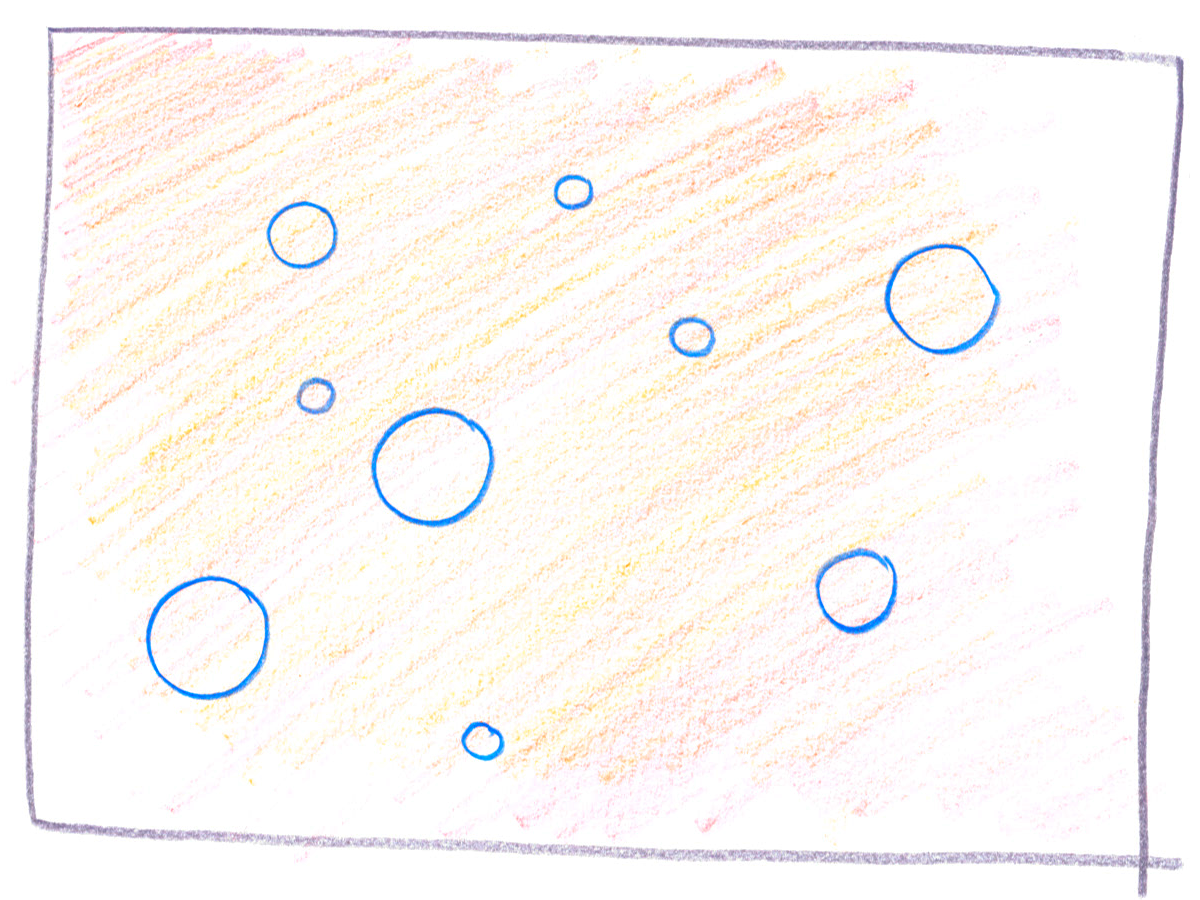
\includegraphics[width=\textwidth]{preliminary/visualizer_idea1.png}
	\caption{A warm, light room with a high level of humidity}
	\label{fig:visualizer_idea1}
\end{figure}

\begin{figure}
	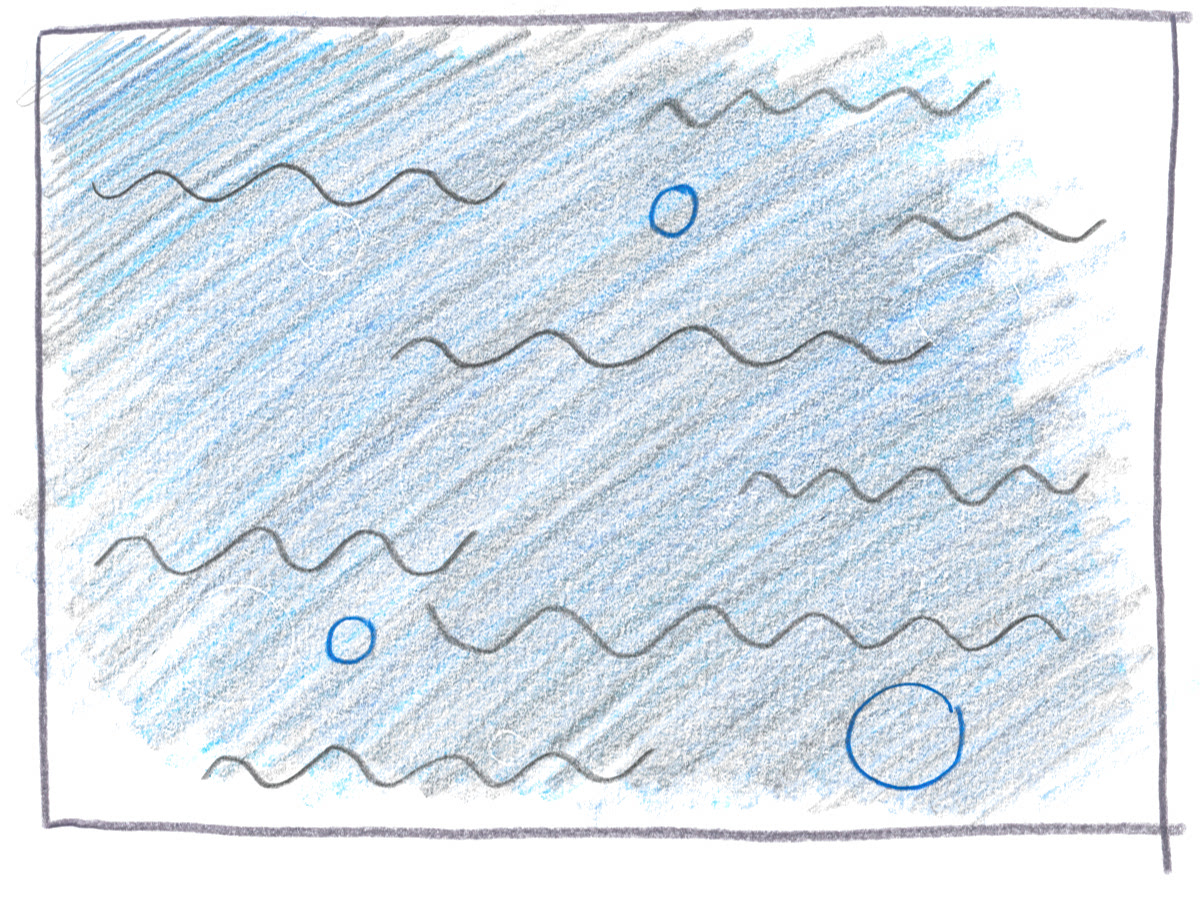
\includegraphics[width=\textwidth]{preliminary/visualizer_idea2.png}
	\caption{A cold, dry and dark room with a high sound level}
	\label{fig:visualizer_idea2}
\end{figure}

This idea is very simple to implement, however, it does not show data per sensor. It shows data as an average, which while it is good for some environments is unacceptable for others. Therefore this idea was quickly abandoned in favour of the next idea.

\subsubsection{Simple Image Manipulation in a Grid}
Instead of having one image that would take all the data and average out the calculations, we would have a grid where a sensor or a group of sensors would provide the same image manipulation but on a grid scale.

While the grid solves the problems of whether individual sensors or a group of sensors are showing, it introduces another major problem. How to make the grid portable and modifiable. This was solved by using grid in a fairly “loose” meaning. Instead of it meaning a grid in its strict sense, the grid would be a sphere around each sensor. In this fashion the system can visualize a sensor’s immediate surrounding as well as average out values that overlap between two spheres. While this adds a layer of complexity to our implementation, we believe that it still remains fairly simple to implement. The ideas are illustrated in  \figref{fig:visualizer_idea3} and in \figref{fig:visualizer_idea4}.

\begin{figure}
	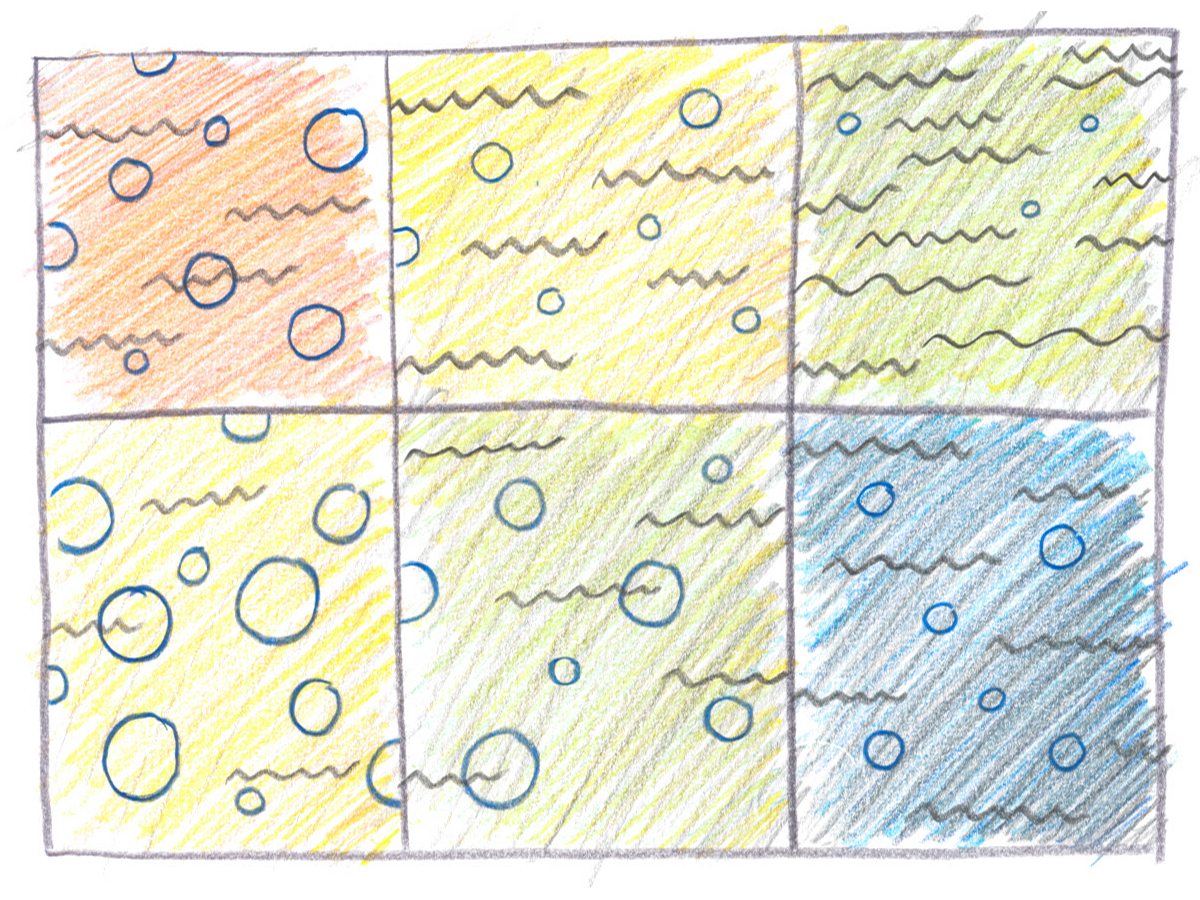
\includegraphics[width=\textwidth]{preliminary/visualizer_idea3.png}
	\caption{Room visualisation with a grid}
	\label{fig:visualizer_idea3}
\end{figure}

\begin{figure}
	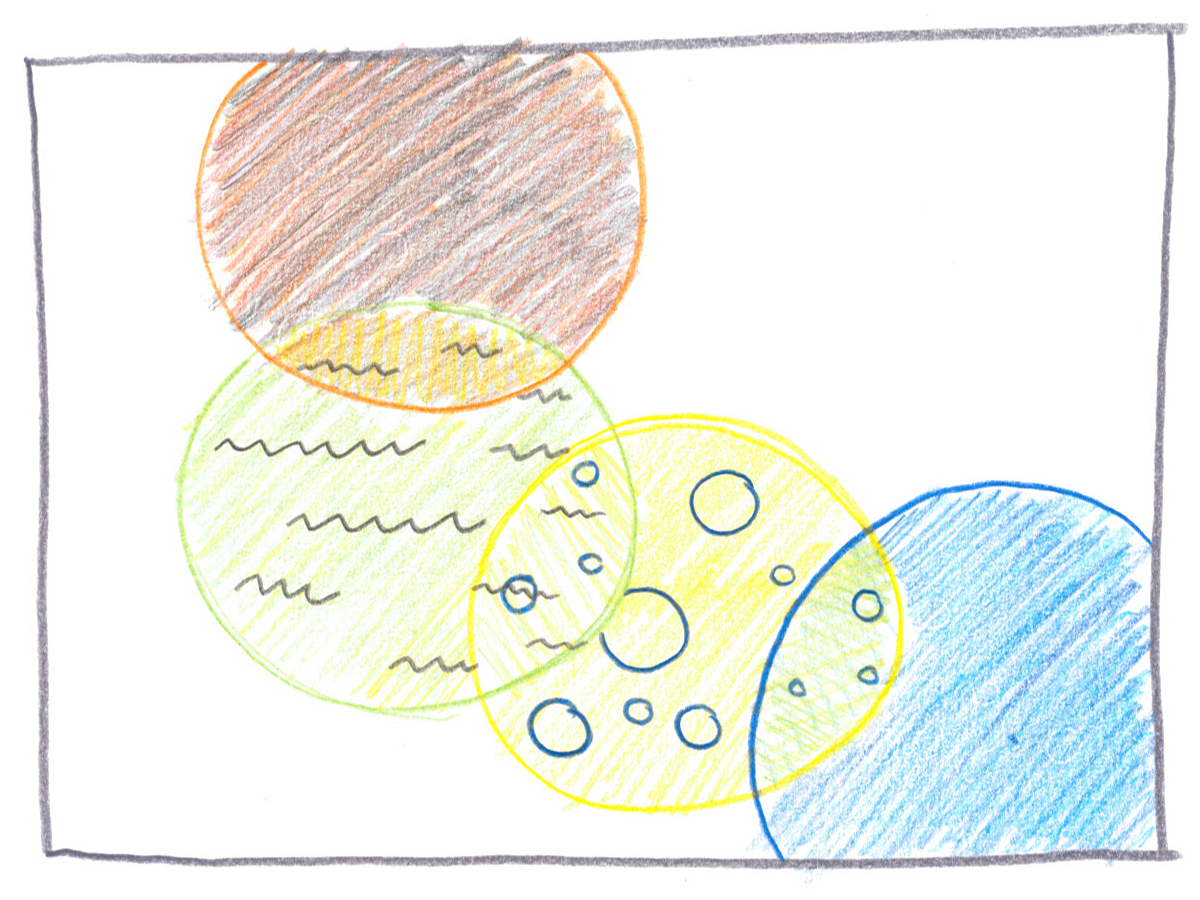
\includegraphics[width=\textwidth]{preliminary/visualizer_idea4.png}
	\caption{Room visualisation with spheres}
	\label{fig:visualizer_idea4}
\end{figure}

\subsection{Manipulation of Sprites}
Instead of using geometrical shapes or simple colours, we can use small pre-made images commonly known as sprites. The system works in quite the same fashion. Every sensor or groups of sensors would be presented by a sprite, which would change based on the changes in the environment.

Sprites may be a bit more intuitive than colours and geometrical shapes, as they can speak more than the shapes can. For example a water sprite rising or lowering could represent the change in humidity. On the other hand it becomes more complex and time consuming to draw the sprites and even potentially animate them. Sprites also may have difficulty representing data that changes slowly, like temperature, and small changes to the data might be difficult to notice. The ideas are illustrated in  \figref{fig:visualizer_idea6} and in \figref{fig:visualizer_idea5}.

\begin{figure}
	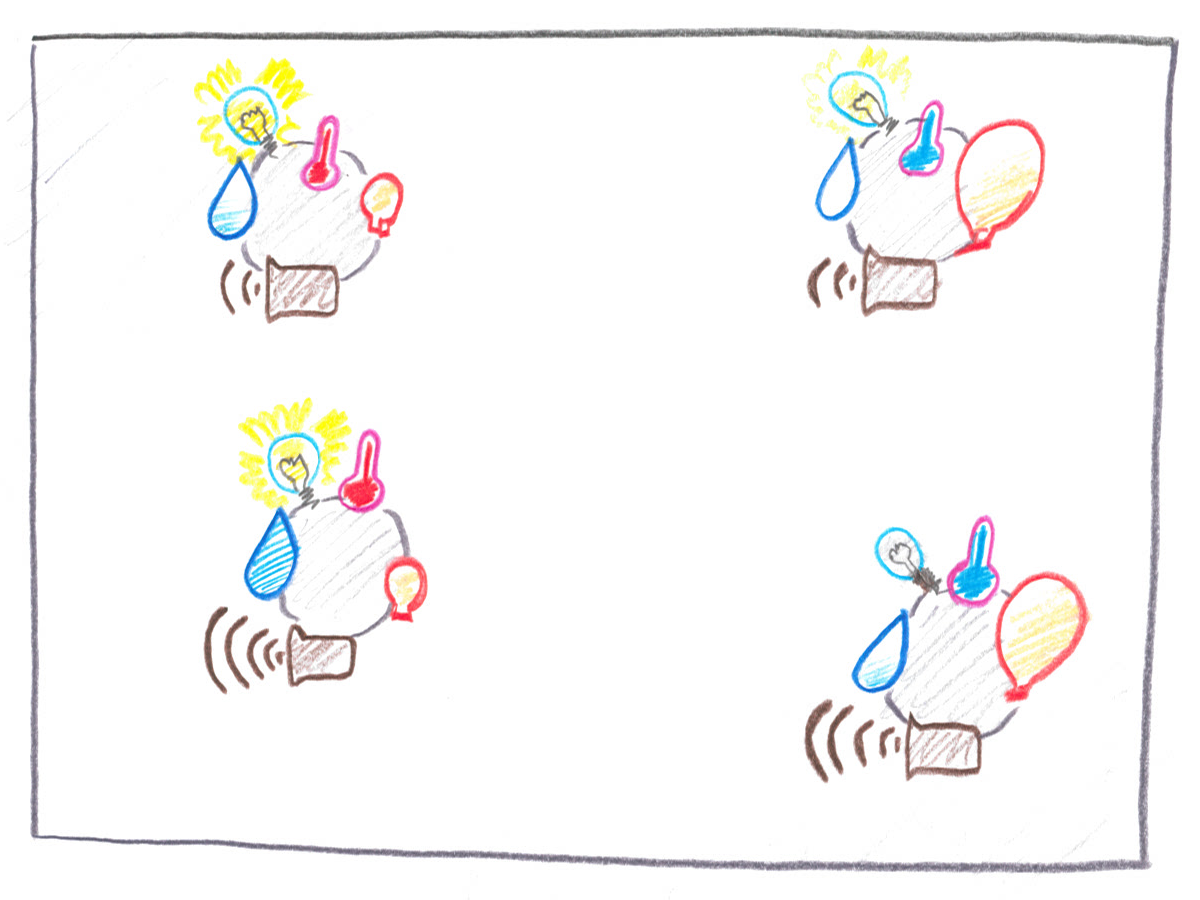
\includegraphics[width=\textwidth]{preliminary/visualizer_idea6.png}
	\caption{Room visualisation with sprites}
	\label{fig:visualizer_idea6}
\end{figure}

\begin{figure}
	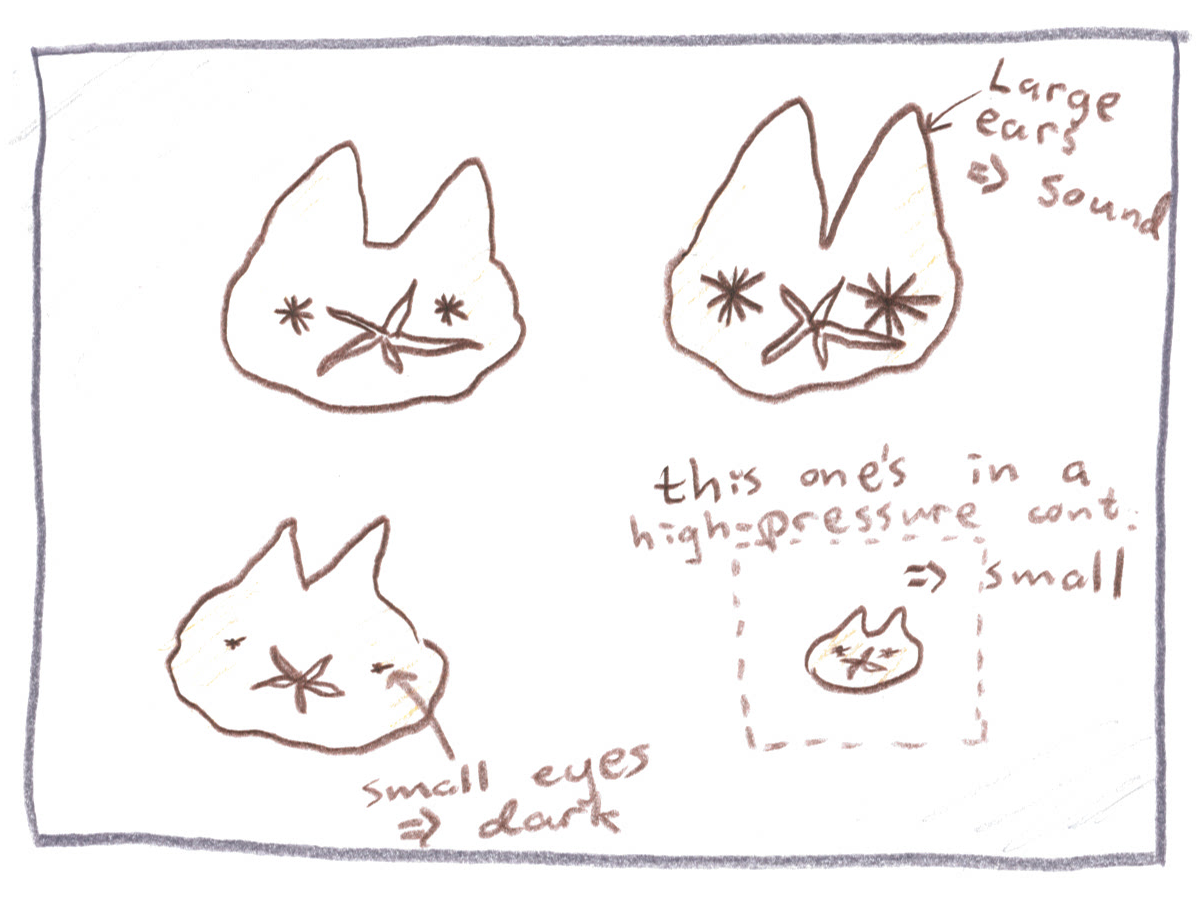
\includegraphics[width=\textwidth]{preliminary/visualizer_idea5.png}
	\caption{Room visualisation with Potato Cat sprites}
	\label{fig:visualizer_idea5}
\end{figure}

\subsubsection{Combination of Sprites and Shapes}

Since sprites may not be able to represent the entire spectrum of data well enough, we could use a combination of sprites and shapes to represent data. Sprites could represent changes that happen more quickly in the environment, such as sound recognition or pressure, while temperature could be represented by colours.

The problem with this approach is that it becomes less intuitive and more cluttered the more we add. While we could make the approach more complex, complexity often hurts intuitiveness. As a result, we would have to carefully balance the two in order to produce a good visual representation. The idea is illustrated in \figref{fig:visualizer_idea7}

\begin{figure}
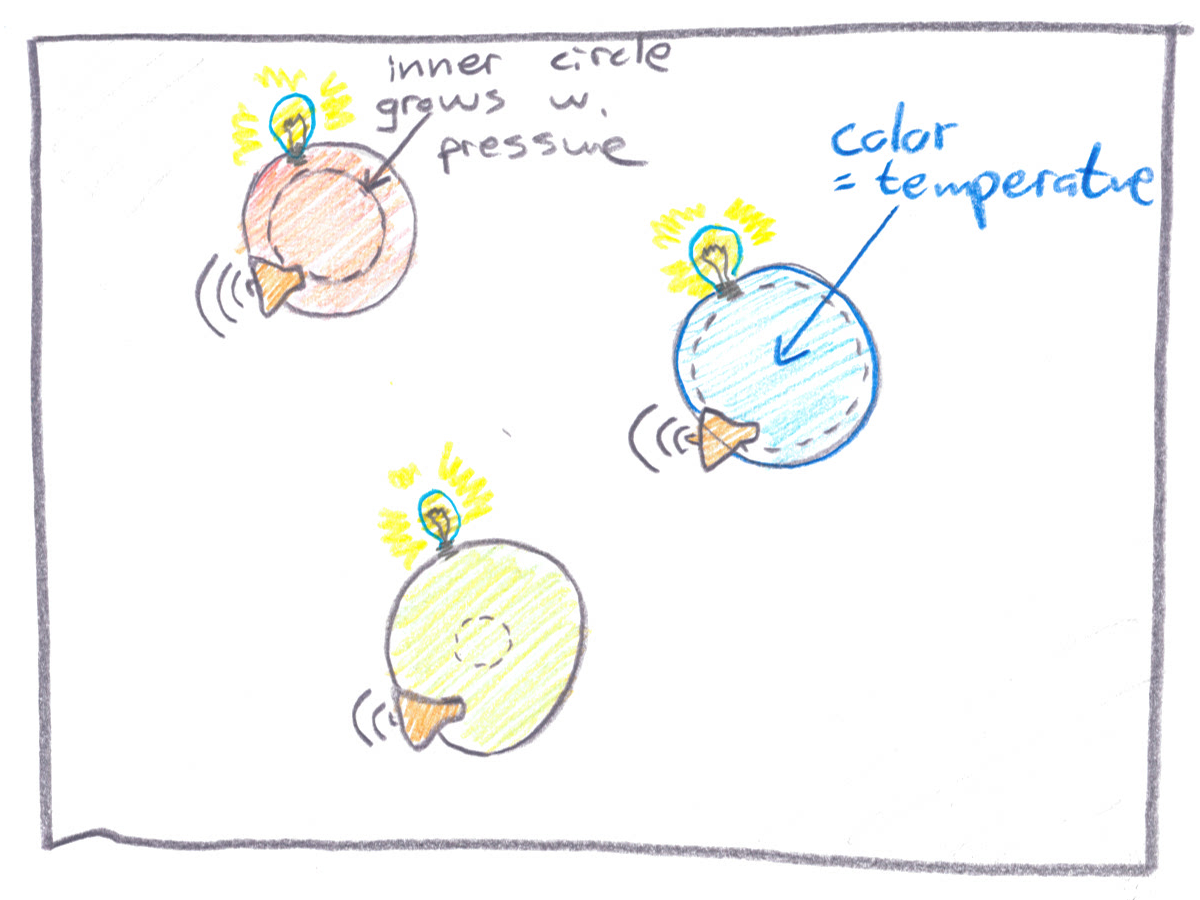
\includegraphics[width=\textwidth]{preliminary/visualizer_idea7.png}
\caption{Room visualisation with sprites and shapes}
\label{fig:visualizer_idea7}
\end{figure}

\subsection{Visualization Ideas Table}
Here we will present the ideas discussed above in the form of a table:

\begin{table}[H]
\centering
\caption{Visualization Ideas Table}
\begin{tabularx}{\textwidth}{|X|X|X|}
	\hline	
	\textbf{Visualization idea}
	&\textbf{Pros}
	&\textbf{Cons}
	\\ \hline Simple Image Manipulation
	&Very simple to implement.
	&Not enough data per sensor is shown.
	\newline \ \newline
	No overarching image of what sensors senses what attribute and the value of the attribute.
	\\ \hline Simple Image Manipulation in a grid
	&Simple to implement.
	\newline \ \newline
	Shows each sensor (or small groups of sensors) and shows their specific attributes.
	&Requires accurate motion tracking to represent the sensors in a 2D environment.
	\\ \hline Manipulation of sprites
	&Adds intuitiveness.
	\newline \ \newline
	Shows each sensor as a sprite and animates the sprite according to the data.
	&The need to animate and draw sprites may be costly in the long run.
	\newline \ \newline
	Some attributes, such as temperature, might not be that intuitive, as they will change very slowly. 
	\\ \hline Combination of sprites and shapes
	&Shows each sensors data clearly and well.
	&Complex implementation.
	\newline \ \newline
	Need to animate and draw sprites may be costly in the long run.
	\newline \ \newline
	Too many sprites and shapes might cause clutter on the screen and actually make it harder to understand.
	\\ \hline 
\end{tabularx}
\end{table}

\subsection{Similar Products and Projects}
\subsubsection{Internet of Things}
The Internet of Things is about connecting devices in our everyday environments to the internet. Many novel uses of internet-connected devices have already been demonstrated, and the future looks promising. It is expected that we will have 100 billion internet-connected objects by 2020. The possibilities might seem limitless. Moreover, the cheap sensor technology supplied by Altran is highly applicable in this area, and such sensors opens up many interesting opportunities.

\subsubsection{Products and Projects}
While there are similar projects that deal with the concept of “Internet of Things”, typically these projects are not limited to the visualization stage. They become a concrete project that uses data to achieve some effect besides visualization. Therefore, most of the products are internal projects that become full fledged projects or products later. It is difficult to find any products that match what we are trying to achieve and most visualizations of data are well out of our field of study, such as weather systems that create cloud or wind patterns and predict their movement.

\subsubsection{The Scrum Model}
\label{the_scrum_model}
The Agile Manifesto and its twelve principles defines a new approach to software development that strongly contrasts with the previous Waterfall model. While the Waterfall model focuses on producing extensive documentation before implementation, an agile development process places the main focus on customer collaboration, presenting working software early, and responding to changes in the product requirements. 

The Scrum model is a framework for software development that closely adheres to the Agile Manifesto. It is an incremental approach in that it develops the product through so-called sprints. A sprint is a phase of implementation that can last from 7 to 30 days. The input to each sprint is the product backlog, which is a list of all product requirements to be implemented ordered by priority. The sprint phase begins with a sprint meeting in which requirements are selected from the backlog to form a sprint backlog. The sprint backlog is the set of requirements that should be implemented during the sprint phase. During the sprint, the development team starts each day with a scrum meeting. Here, each team member presents what was done yesterday, what should be done today, and if there are any difficulties. The sprint ends with an end meeting in which the work progress is evaluated, and a demo of the new product increment is presented to the stakeholders.

In our initial project phase, we do not follow the Scrum model strictly. The initial phase is more concerned with documenting product requirements. This work would benefit from a close collaboration with the customer, making us choose our own agile model of work. In addition to having regular customer meetings, we opened up all our product documentation to the customer. The customer was prompted by email to review new versions of documents so that he could provide feedback outside meeting hours.

During the implementation phases, the Scrum model will be much more central. Here we will apply it to have a backlog, scrum meetings, and sprints.

\subsubsection{Different Possible Architectural Models for the Prototype}
While working on the initial stages of the project, we had to prepare countermeasures to counteract risk 1, as seen in the risk table under \subsubfullref{risks_and_risk_mitigation}, which was the possibility of us not getting the hardware necessary to complete our prototype. In order to make the prototype work without any hardware from the customer, he suggested that we could substitute the sensors with android phones. With this in mind we had to prepare for both situations and we found out that the architecture in both cases actually differs. In both cases we would be using a client-server architecture, however, the roles of the client and the server would be reversed.

When using the sensors, we would have a raspberry pi acting as a server. In this case our client requests information from the server, and stores it in a database of some sort. Then our visualizer uses this data to show it in a visual way. The image of the architecture can be seen below.

\begin{figure}[H]
	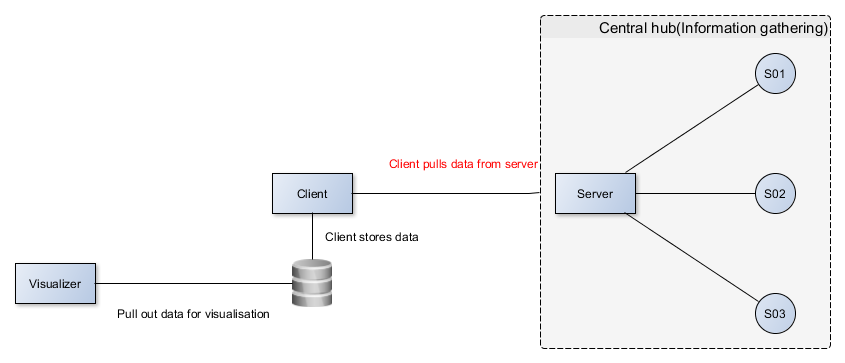
\includegraphics[width=\textwidth]{preliminary/Architecture_1.png}
	\caption{Architecture Solution 1}
\end{figure}

The architecture that deals with the android phones is the opposite. The phones are sensors, but also servers at the same time, and we have only one client, that requests information from the phones, or servers. This information is stored in some sort of a database, and the same process is repeated as above with the visualizer. The image of the architecture can be seen below.

\begin{figure}[H]
	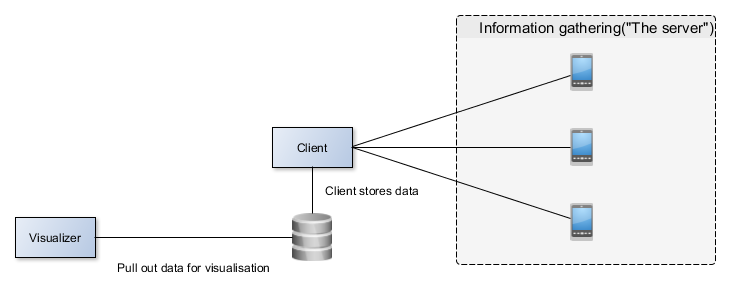
\includegraphics[width=\textwidth]{preliminary/Architecture_2.png}
	\caption{Architecture Solution 2}
\end{figure}

The two architectures are both client server, but they are quite different as can be seen from the images. They are both worth mentioning, as they will influence our implementation based on the hardware provided.

\subsection{Tools}
Below we will list the major tools we will use to create our project. This encompasses both the hardware that we will be using as well as major programming languages or protocols that we will use to complete this project. The full list of tools used can be found in appendix A.

\subsubsection{Hardware}
As stated before, we need to prepare for both architectures. The hardware then encompasses both the sensors and the android phones. We will also note down the DASH7 standard for wireless networking, which is used by the sensors.

\subsubsection{Sensors}
We were given a short demonstration of the sensor capabilities by the customer on our first meeting. We know that the sensors are able to detect temperature, pressure, humidity and light. It also has a built in accelerometer. The sensors also have two led lights, one green and one red, that can be remotely turned on or off, although they are not very interesting in our project, the lights can be used in different projects. There is also a large (comparative to the sensor) antenna mounted at the end of the sensor. The sensors use DASH7 standard (explained below in more detail) to connect to a central hub of some sort. From a client we are then able to view and extract this information. The sensors are quite small in size, even with an antenna they are not more than 15 centimetres long and 5 centimetres wide, with a thickness (including the antenna) of about 1-2 centimetres. The sensors are quite cheap to manufacture as well. The sensors should be provided to us by the customer when we start working on the implementation.

\subsubsection{Android phone}
In the case that we would not receive sensors, we could use android phones. An android phone works very similar to our sensors. The sensors that exist on the android phone can measure light, ambient temperature, pressure, humidity, proximity, gravity and acceleration to the device. The data gathering process would be done through an application, commonly also referred to as an app, that would run in the background, listen for requests and reply with data. This app would be written Java, as it is the main programming language for android phones. Except for humidity, all of the other sensors were implemented as of android 2.3.

\subsubsection{DASH7}
DASH7 is a RFID-standard for wireless networking, that operates on 433 Mhz unlicensed SRD band. It provides long battery life, up to 2 km connection distance, low latency with moving objects and 1 metre accuracy. It is frequently used in the military.

No one in our group is familiar with DASH7, therefore we needed to spend at least some time studying it’s capabilities. It is not an overly important part of the system, after the only concern that we have with it is in between the sensors and the central hub, the part of the system we will not modify in any fashion. Still it is worth mentioning as a separate part of hardware, since it demonstrates the network capability of the sensors in comparison to standard WiFi networking and also demonstrates further the capabilities of the sensors.

\subsubsection{Software}
In this project we will mainly be using Java as a programming language. We will also use LaTeX for formatting our presentation into a more presentable and clean document.

\subsubsection{Java}
Java is a high level, class-based, object-oriented programming language, introduced in 1995. There are two major advantages for using Java in our system. The first one is that the entire development team is familiar with the Java programming language and we do not have to spend time learning to program in Java. The second advantage is in it’s class-based, object-oriented design. It allows us to work in pairs on classes, and allows classes to synchronize better with each other, so it makes programming easier. Not only that, but Java also has some very good ways of implementing a user interface, such as JavaFX, which will help us visualize the project easier. Since visualization is the main goal, Java is, we feel, an excellent choice of programming language for this project.

\subsubsection{\LaTeX}
LaTeX is a document markup language. LaTeX is widely used in document preparation, as it has many functions that improve the readability of the document, as well as many automatic functions such as generation of a table of contents and chapter numbering. It also has a clean and consistent way of presenting tables as well as symbols for any kind of mathematical formula. At least half of our team is familiar with LaTeX and it is a markup language that is fairly easy to learn, in our opinion, so it will not constrain our time further. In fact, with the automatic table and diagram marking it will make our document much more readable and presentable and that is why we choose to use it.
















\end{document}